\subsection{Ist-Analyse}

Wie bereits unter Ausgangssituation beschrieben, wird derzeit eine veraltete und unübersichtliche / fehleranfällige \gl{MED} zur Erstellung der \gl{RA} verwendet. Der Prozess zur Einreichung einer \gl{RA} wird im folgenden Abschnitt \sct{sec:Analysephase:Reisekostenabrechnungsprozess}{Reisekostenabrechnungsprozess} näher erläutert.

\subsubsection{Reisekostenabrechnungsprozess}
\label{sec:Analysephase:Reisekostenabrechnungsprozess}

Der \gl{MA} im Außendienst füllt die \gl{RA} aus und legt sie seinem Vorgesetzten (und ggf. der \gl{GF}) vor, welche prüfen, ob die Dienstreise(n) genehmigt wurde(n). Ist dies der Fall, wird die an die Payroll Accounting Abteilung weitergeleitet und dort auf Manipulationen überprüft. Weist die \gl{RA} keine Manipulationen vor, kann sie an die Accountig Abteilung weitergeleitet werden, die die Berechnungen und die Übereinstimmung der Belege mit den eingetragenen Kosten überprüft. Ist die \gl{RA} in Ordnung, kann eine entsprechende Auszahlung veranlasst werden. Sollte jedoch in einem der oben genannten Fälle etwas mit der \gl{RA} nicht in Ordnung sein, muss diese vom Mitarbeiter bearbeitet werden oder wird schlichtweg abgelehnt.

Eine grobe Darstellung des aktuellen Reisekostenabrechnungsprozesses ist in visueller Form im Anhang unter \sct{sec:Anhang:ProzessAlt}{Prozess Alt} zu finden.

\subsubsection{Herausforderungen}

Wie in der \sct{sec:Einführung-Definitionsphase:Ausgangssituation}{Ausgangssituation} beschrieben, ist diese \gl{MED} komplex, was zu Fehlern führt, wie z.B. dass Bedingungen falsch verstanden werden und dementsprechend eingetragen werden, obwohl sie nicht eingetragen werden sollten. Grundsätzlich kann es aufgrund der Art der \gl{MED} zu Manipulationen der Berechnungslogik oder der Pauschalen kommen. Zudem kommt es häufig vor, dass notwendige Belege nicht beigefügt werden oder die angegebenen Kosten nicht validiert werden können. Diese Herausforderungen erschweren den Einsatz in den Abteilungen, in diese verwendet wird.

\subsection{Wirtschaftlichkeit}
Da diese Softwarelösung die veraltete \gl{MED} ablösen soll, spielt die Wirtschaftlichkeit eine untergeordnete Rolle. Dennoch können monatliche Einsparungen erzielt werden, die sich anhand folgender Annahmen/Durchschnittswerten ergeben.

Von folgenden Personalkosten wird ausgegangen:
\begin{itemize}
\item Azubi/Autor: 7€
\item \gl{MA} im Außendienst: 25€
\item Junior Software Developer: 27€ 
\item Accounting Abteilung/ Payroll Accounting/ Betreuerin: 30€
\item Vorgesetzter: 45€
\item \gl{GF}: 100€
\end{itemize}

Folgende Annahmen gelten universell:
\begin{itemize}
\item 20 \glp{RA} werden im Monat eingereicht
\item Genehmigung des Vorgesetzten - 1 Vorgesetzter à 5 Minuten
\item Genehmigung der \gl{GF} - 1 \gl{GF} einmal im Monat à 5 Minuten
\item 10\% der Ersteller wenden sich mit Fragen direkt an die Account Abteilung - 1 \gl{MA} Accounting, 1 \gl{MA} im Außendienst à 10 Minuten
\end{itemize}

Folgende Annahmen gelten für den Prozess rund um die \gl{RA} mit der bestehenden \gl{MED}:
\begin{itemize}
\item \gl{RA} erstellen - 1 \gl{MA} im Außendienst à 15 Minutent
\item Jeden 2. Monat Einführung eines \gl{MA} - 2 \gl{MA} im Außendienst à 1 Stunde
\item 20\% der Ersteller bitten Kollegen um Hilfe - 2 \gl{MA} im Außendienst à 15 Minuten
\item 90\% der \gl{RA} wird über die Hauspost geliefert - 1 Azubi à 10 Minuten
\item 10\% der \gl{RA} wird selbst gebracht – 1 \gl{MA} im Außendienst à 10 Minuten
\item Prüfung auf Manipulation - 1 \gl{MA} Payroll Accounting à 10 Minuten
\item Prüfung auf Richtigkeit - 1 \gl{MA} Accounting à 12 Minuten
\item 25\% der \glp{RA} müssen korrigiert werden – 1 \gl{MA} im Außendienst à 10 Minuten
\item 25\% der \glp{RA} müssen nachgeprüft werden - 1 \gl{MA} Accounting à 7 Minuten
\end{itemize}

Summe der Monatlichen Kosten/Verluste durch die Aktuelle Lösung: 589,33 €

Folgende Annahmen gelten für den Prozess rund um die \gl{RA} mit der Neu entwickelten Softwarelösung Travel-Assistant:
\begin{itemize}
\item \gl{RA} erstellen - 1 Mitarbeiter im Außendienst à 20 Minuten
\item 10\% der Ersteller bitten Kollegen um Hilfe - 2 \gl{MA} im Außendienst à 5 Minuten
\item Prüfung auf Richtigkeit - 1 \gl{MA} Accounting à 7 Minuten
\item 10\% der \glp{RA} müssen korrigiert werden – 1 \gl{MA} im Außendienst à 7 Minuten
\item 10\% der \glp{RA} müssen nachgeprüft werden - 1 \gl{MA} Accounting à 5 Minuten
\item Wartung der Softwarelösung – 1 Junior Software Developer à 2 Stunden
\end{itemize}

Summe der Monatlichen Kosten/Verluste durch die Neuentwickelte Softwarelösung: 411,50€

Monatliche Kosten Ersparnis: 177,83€

Entwicklungskosten des Travel-Assistant:
\begin{itemize}

\item Implementierung - Autor à 80 Stunden
\item Hilfestellung/Rat - Betreuerin à 5 Stunden 
\item Meetings/Abnahme und diverse Rückfragen - 1 Autor, 2 \gl{MA} Accounting à 6 Stunden
\item Feedback/Testing - 1 \gl{MA} im Außendienst à 1 Stunde
\end{itemize}

Summe Projekt Entwicklungskosten: 1.095,00€

Damit die Softwarelösung Vollumfänglich eingesetzt werden kann muss diese um einige Features weiterentwickelt werden, siehe Ausblick. Angenommen wird:
\begin{itemize}
\item Weiterentwicklung - 1 Junior Software Developer à 25 Stunden
\item Zusätzliche Meetings - 1 Junior Software Developer, 2 \gl{MA} Accounting à 4 Stunden
\end{itemize}

Summe Entwicklungskosten bis zum Vollumfänglich einsatz : 1.023,00 € (2.118,00 €)

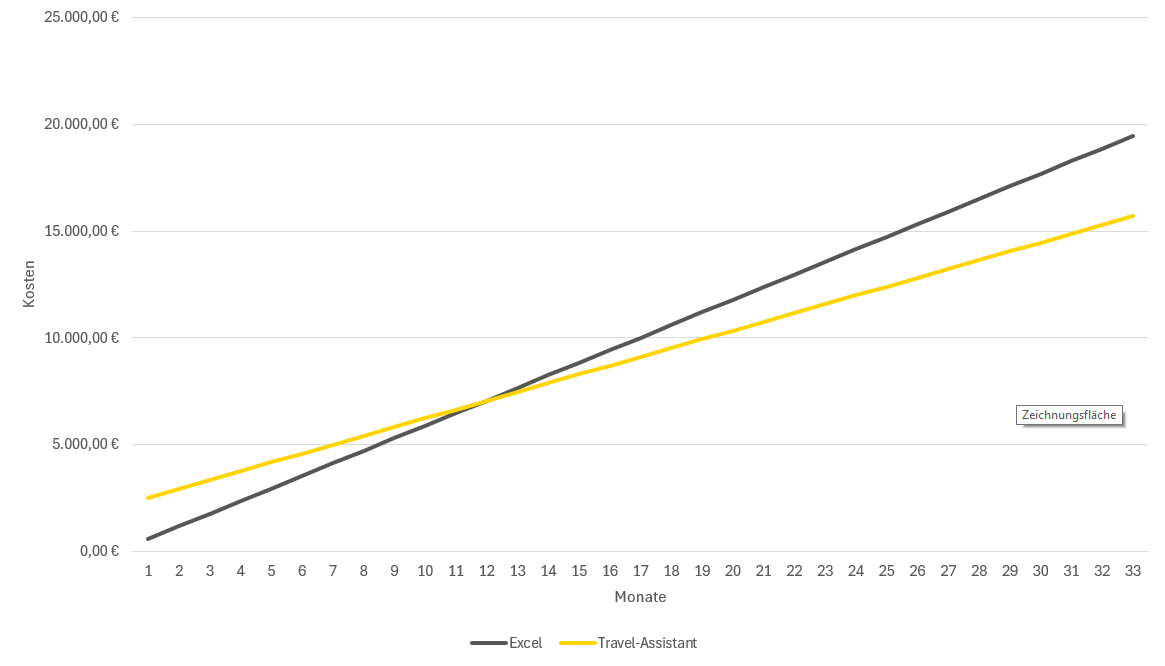
\includegraphics[width=1\textwidth]{amortisationsrechnung.png}

Damit ergibt sich ein Break Even Point bei ungefähr 12 Monaten.

Diese Annahmen basieren auf Durchschnitts- oder Erwartungswerten, von denen realistischerweise ausgegangen werden kann.
Detailierte Berechnung ist im Anhang unter \sct{sec:Anhang:Amortisationsrechnung}{Amortisationsrechnung} zu finden.

\subsection{Anwendungsfälle und Benutzerklassifizierung}
\label{sec:Analysephase:Benutzerklassifizierung}

Um herauszufinden, wie das Berechtigungskonzept aussehen sollte, wurde analysiert, welche Personengruppen wie mit der Softwarelösung arbeiten müssen.
Grundsätzlich lassen sich folgende drei Personengruppen feststellen:

\begin{enumerate}
    \item \emph{Reguläre Benutzer}\\
    Jede mitarbeitende Person, die berechtigt ist, \glp{RA} einzureichen.
    \item \emph{Vorgesetzte/\gl{GF}}\\
    Personen, die berechtigt sind, \glp{RA} anderer Personen zu bestätigen.
    \item \emph{Prüfer}\\
    Personen, die berechtigt sind, \glp{RA} auf ihre Richtigkeit zu prüfen.
\end{enumerate}

Im Anhang ist ein \sct{sec:Anhang:Anwendungsfalldiagramm}{Anwendungsfalldiagramm} zu finden welches möglichen Aktionen der Jeweiligen Personengruppen zuordnet.